\section{01. Mai 2015}
\question{Austauschenergie beim \ch{H2}-Molekül? Wann ist es groß/klein? Wieso ist es für die Bindung wichtig?}
\label{q:1}

Die Austauschenergie oder oft auch \textbf{Austauschwechselwirkung} spielt bei der chemischen Bindung eine bedeutende Rolle.

Sie ist groß, falls sich die Atomorbitale stark überlappen -- sprich symmetrisch sind -- und kleiner, falls sie sich weniger überlappen (=anti-symmetrisch).

Wie man in der Abbildung erkennen kann, ergibt sich eine Bindung nur, wenn die Orbitale sich überlappen (im symmetrischen Fall $U_S$).

\begin{figure}[H]  
    \centering
    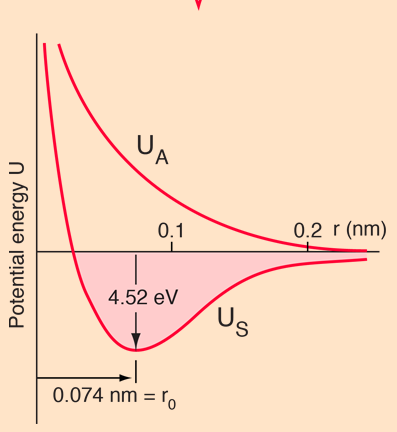
\includegraphics[width=.4\textwidth]{resources/05-01-2015/Frage1.png}
    \caption{siehe \href{http://hyperphysics.phy-astr.gsu.edu/hbase/molecule/hmol.html}{LINK}}
\end{figure}

\question{Was kann man aus dem Rotations-Schwingungsspektrum für molekulare Größen bestimmen?}
\label{q:2}

Unter Annahme, dass die beiden Atome ihren Abstand bei Rotation nicht ändern, kann man den \textbf{Bindungsabstand} $R_e$ bestimmen. \\
Weiter lässt sich die \textbf{Rotationskonstante} $B_e$ bzw. deren anharmonischer Anteil $\alpha_e$, die \textbf{Schwingungsfrequenz} $\omega$ und das \textbf{Trägheitsmoment} $I$ bestimmen. \\

\[B_e = \frac{\hbar}{4 \pi c M R_e^2}\text{\quad [cm$^{-1}$]}\]
\[E_{rot} = \frac{\hbar^2}{2 I} \cdot J(J+1)\text{\quad [J]}\]
\[E_{rot} = B_e \cdot h\cdot c\]
$J$ ist dabei die Quantenzahl der Rotation und $M$ die reduzierte Masse (damit $M * R_e^2$ eben $I$ entspricht; gilt freilich nur für 2-Atom Systeme). \\

\[\Delta E_{rot} = \frac{\hbar^2}{M R_e^2}(J+1) = 2B(J+1)\]
\[\Delta E_{vib} = \hbar \cdot \omega\]

\question{Diskutieren Sie elektrische Rotations-Schwingungsübergänge und die Entstehung von Schwingungsbanden.}
\label{q:3}

Übergänge zwischen Schwingungs-Rotations-Niveaus ($f_i$,$J_i$) $\rightarrow$ ($f_j$,$J_j$) innerhaltb desselben elektronischen Zustandes bilden für $f_i \neq f_j$ ein Schwingungs-Rotations-Spektrum. \\

\textbf{WICHTIG:} nur Moleküle welche ein permanentes Dipolmoment besitzen können solche Übergänge durchführen (z.B.: \ce{CO2}, \ce{H2O} aber \underline{nicht} \ce{O2}, andere homonuklearen, \dots etc.). \\

Wird Energie (Photon) von außen zugeführt oder abgegeben, so kann ein Übergang zwischen den Niveaus stattfinden - Auswahlregel $\Delta J = \pm 1$. Sprich Rotations-Schwingungsübergänge spielen sich zwischen benachbarten Niveaus ab.\\

\textbf{Schwingungsbanden} bezeichnen nun alle Rotationslinien welche zu einem Schwingungsübergang gehören. \\


\question{Was für ein Zusammenhang besteht zwischen der Gitterebene und einem Vektor im reziproken Raum?}
\label{q:4}

Der Abstand zweier Gitterebenen $d_{hkl}$ ist gegeben durch:
\[d_{hkl} = \frac{1}{\sqrt{\left(\frac{h}{a}\right)^2 + \left(\frac{k}{b}\right)^2 + \left(\frac{l}{c}\right)^2}}\]
und hängt mit dem reziproken Gittervektor $\vec{G_{hkl}}$ 
\[\vec{G}_{hkl} = h\vec{b}_1 + k\vec{b}_2 + l\vec{b}_3\]
wie folgt zusammen:
\[d_{hkl} = \frac{2\pi}{|\vec{G_{hkl}}|}\]

Somit ist die Länge des reziproken Gittervektors $\vec{G_{hkl}}$ indirekt proportional zum Abstand der Gitterebenen $d_{hkl}$.

\question{Erklären Sie das Auftreten von Energiebandlücken mithilfe des Models der fast freien Elektronen.}
\label{q:5}

Als Bandlücke wird der energetische Abstand zwischen Valenzband und Leitungsband eines Festkörpers bezeichnet. Dessen elektrische und optische Eigenschaften werden wesentlich durch die Größe der Bandlücke bestimmt.
Nach dem Bändermodell sind gebundene Zustände der Elektronen nur auf bestimmten Intervallen der Energieskala zugelassen: den Bändern. Zwischen den Bändern können energetisch verbotene Bereiche liegen. Jeder dieser Bereiche stellt eine Lücke zwischen den Bändern dar, jedoch ist für die physikalischen Eigenschaften eines Festkörpers nur die eventuelle Lücke zwischen dem höchsten noch vollständig mit Elektronen besetzten Band und dem nächsthöheren von entscheidender Bedeutung.

Daher ist mit der Bandlücke immer diejenige zwischen Valenz- und Leitungsband gemeint.
Das Auftreten einer solchen Lücke lässt sich durch das Modell der quasifreien Elektronen beschreiben. Dabei wird das Modell freier Elektronen, welches das Verhalten der Valenzelektronen in einer kristallinen Struktur eines festen Metalls darstellt, durch ein elektrostatisches periodisches Potential
erweitert.
\begin{equation}
    \label{eq:coulomb_potential}
    V_0(r) = \frac{1}{4\pi\epsilon_0}\frac{q}{r}
\end{equation}
Die freien Elektronen werden durch diese anziehende Coulomb-Wechselwirkung jedoch nur wenig gestört, da zusätzlich zu dieser anziehenden eine abstoßende Wechselwirkung aufgrund des Pauli-Prinzips auftritt. Beide WW sind im Bereich der Atomrümpfe am stärksten.

Zusätzlich wird die anziehende Wechselwirkung der Atomrümpfe durch die freien Elektronen des Elektronengases abgeschirmt. Diese abschirmende Wirkung wird durch einen Korrekturterm im Coulomb-Potential beschrieben.
\begin{equation}
    \label{eq:}
    V(r) = \frac{1}{4\pi\epsilon_0}\frac{q}{r}e^{-r/r_{\text{TF}}}
\end{equation}
Dabei beschreibt $r_{\text{TF}}$ den Thomas-Fermi-Radius, welcher den Abstand beschreibt, ab dem die anziehende Wechselwirkung stark nachlässt.
\begin{equation}
    \label{eq:Thomas-Fermi-Radius}
    r_{\text{TF}} = \frac{a_0}{2}\left(\frac{\pi}{\sqrt{3}}n\right)^{\frac{1}{6}},
\end{equation}
mit $a_0$ als den Bohr-Radius.

\begin{figure}[H]
    \centering
    \begin{samepage}
        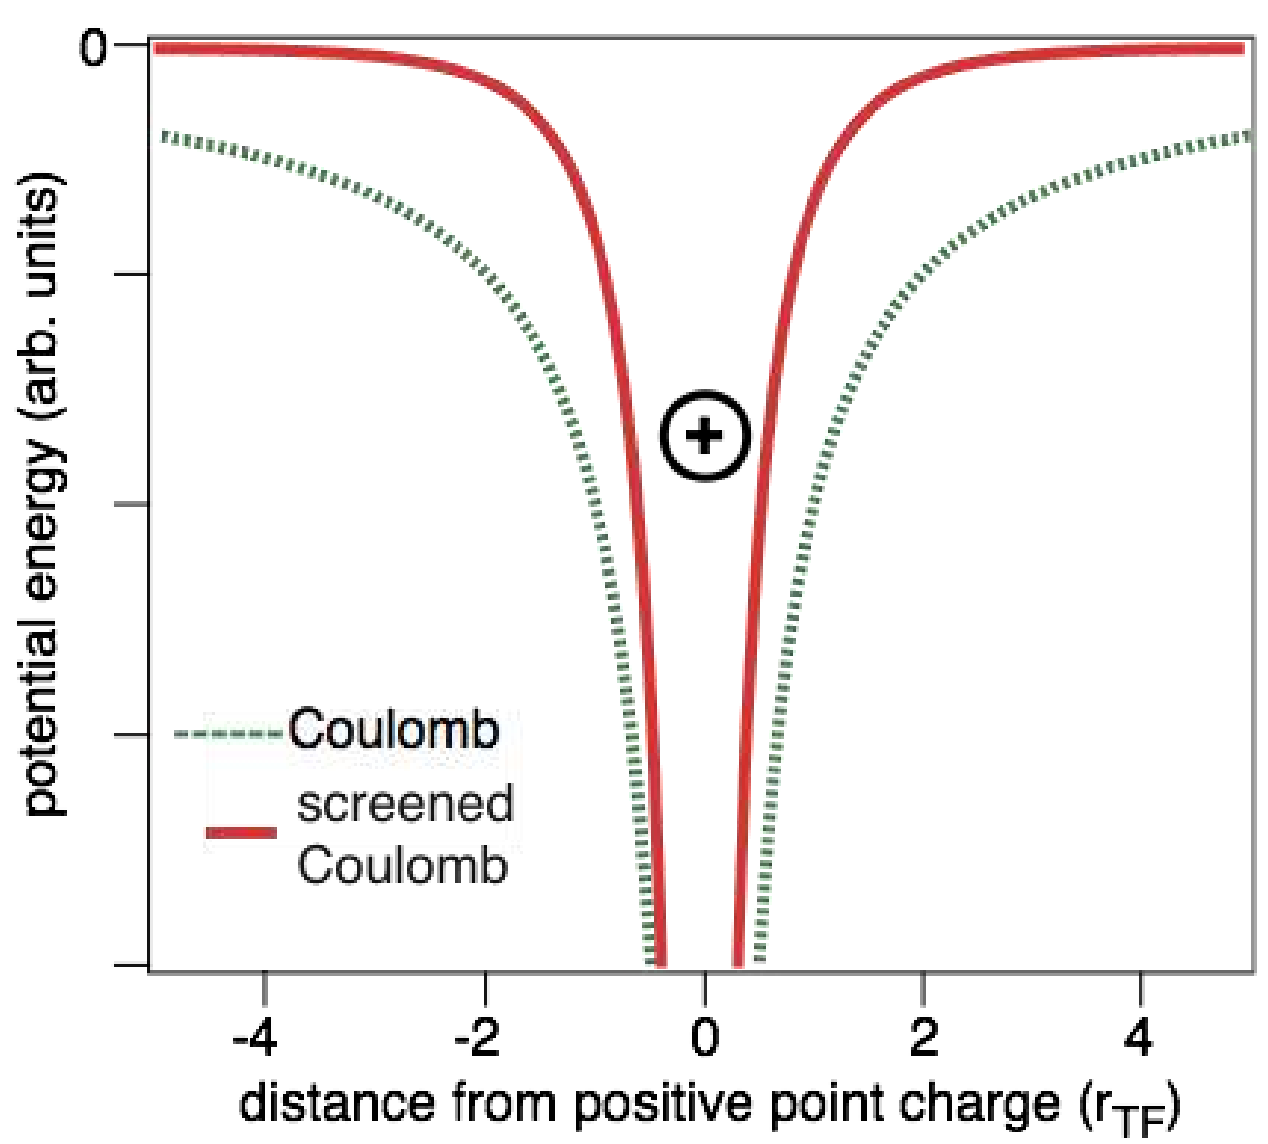
\includegraphics[width=0.6\linewidth]{resources/05-01-2015/coulomb_potential_screened.png}
        \caption{Coulomb-Potential und abgeschirmtes Coulomb-Potential im quasifreien Teilchenmodell}
        \label{fig:coulomb_potential_with_and_without_screening}
    \end{samepage}
\end{figure}

Dadurch kommt es zu einer näherungsweisen Beschreibung der positive geladenen Atomrümpfe im Kristallgitter. Man setzt dabei zunächst die Periodizität der Energiebänder im reziproken Raum an, welche bei Berücksichtigung eines kleinen Gitterpotentials an den Zonengrenzen eine Bandlücke aufweisen. 
Diese Methode erlaubt eine theoretische Vorhersage der Bandlücke und damit eine Einteilung der Festkörper in elektrische Leiter, Halbleiter und Isolatoren.
Hierbei gilt als Faustregel:

\begin{itemize}
    \item \textbf{Leiter:} keine Bandlücke.
    \item \textbf{Halbleiter:} Bandlücke im Bereich von 0,1 bis ca. 3 eV.
    \item \textbf{Nichtleiter:} Bandlücke größer als 3 eV.
\end{itemize}

\question{Wie kann experimentell die Dispersionsrelationskurve von Phononen ermittelt werden?}
\label{q:6}

\begin{enumerate}
    \item Neutronen auf Kristallgitter schießen
    \item Impuls der Neutronen vorher und nachher messen
    \item Durch Energieverlust auf Phononen schließen
\end{enumerate}

\begin{figure}[H]  
    \centering
    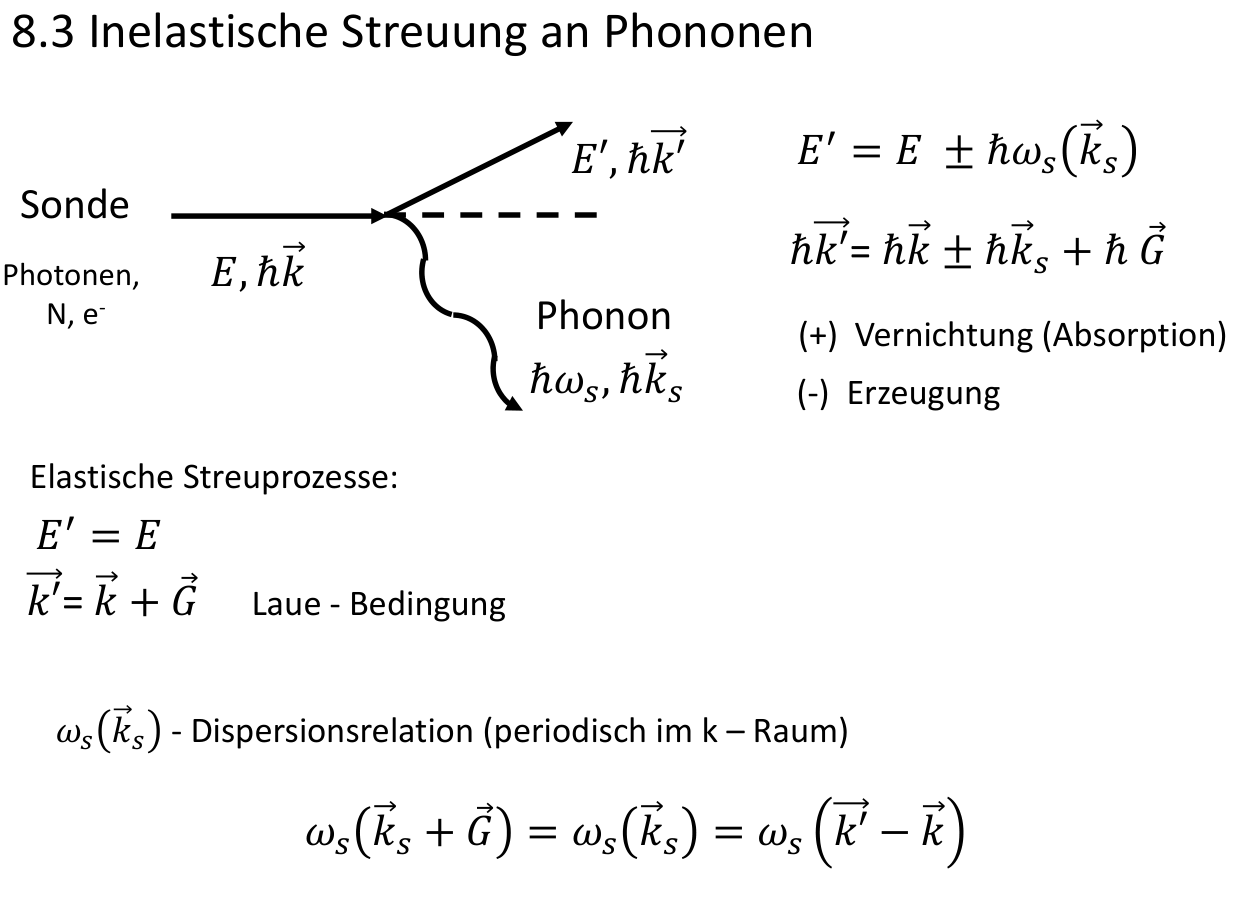
\includegraphics[width=.8\textwidth]{resources/05-01-2015/Frage6_1.png}
    \caption{Inelastische Streuung an Phononen}
\end{figure}

\begin{figure}[H]  
    \centering
    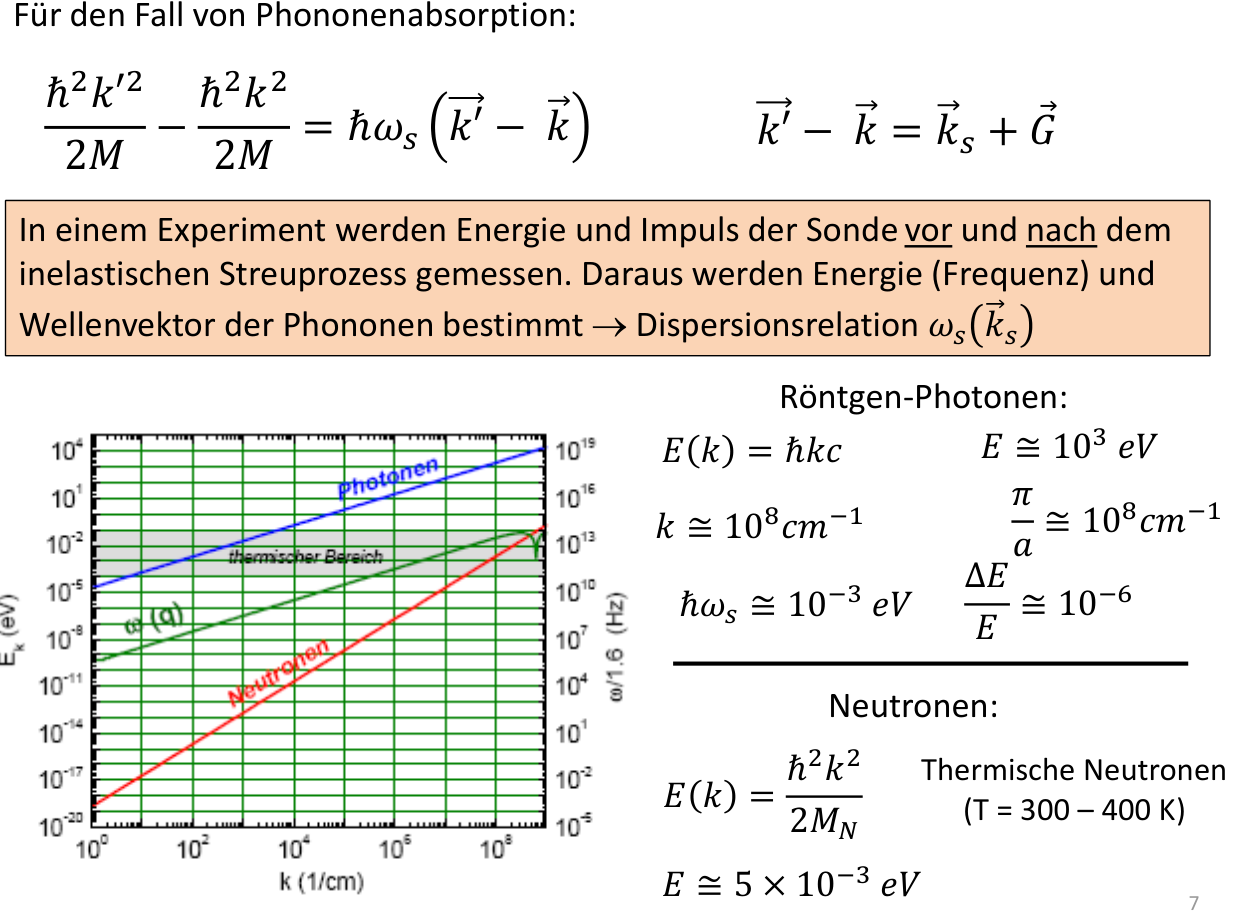
\includegraphics[width=.8\textwidth]{resources/05-01-2015/Frage6_2.png}
    \caption{Dispersionsrelation Phononen in einem Experiment}
\end{figure}

\question{Diskutieren Sie die Wärmekapazität sowohl in der klassischen als auch in der quantenmechanischen Betrachtung.}
\label{q:7}

In der der klassischen Physik wird angenommen, dass die Energieauf- und abnahme eines Materials 
kontinuerlich ist bzw. die Energieniveaus von Molekülen und Atomen eines Materials kontinuierlich 
variieren können. \\
In den quantenmechanischen Modellen können die Energieniveaus nur diskrete Werte annehmen, wodurch die 
Wärmekapazität eines Materials bei niedrigen Temperaturen diskrete Schritte 
aufweist, die durch die Energieniveaus der quantenmechanischen Zustände bestimmt sind (Einstein, Debye).
(Die Quantisierung der Gitterschwingungen ist entscheidend für die innere Energie und
die spezifische Wärme des Kristallgitters.)
\\
Bei hohen Temperaturen nähert sich die klassische Wärmekapazität der quantenmechanischen Wärmekapazität 
an (Abstände zwischen Energieniveaus wird kleiner).

\begin{figure}[H]  
    \centering
    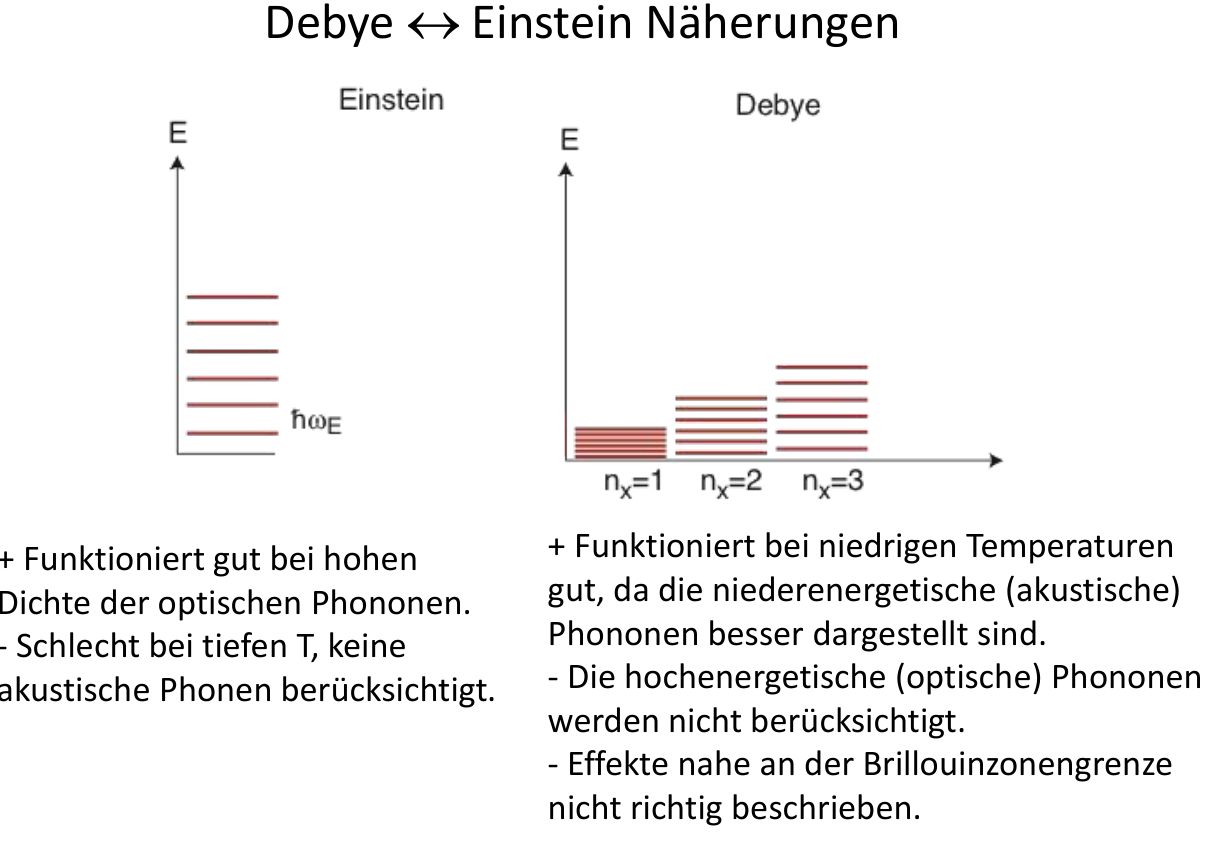
\includegraphics[width=.8\textwidth]{resources/05-01-2015/Frage7.png}
    \caption{Vergleich zwischen Einstein- und Debye-Modell.}
\end{figure}

\question{Beschreiben Sie das Bloch-Theorem eines Elektrons im harmonischen Potential.}
\label{q:8}

Das Bloch-Theorem beschreibt das Verhalten eines Elektrons in einem periodischen Potential. Dabei nimmt das Elektron eine spezielle Wellenfunktion an, die als Bloch-Funktion bezeichnet wird. Diese Bloch-Funktion hat die Form einer ebene Welle multipliziert mit einer periodischen Funktion, die die Symmetrie des Potentials widerspiegelt.

Im Fall eines harmonischen Potentials ergibt sich die Schrödinger-Gleichung für ein Elektron zu:
\begin{align}
 \left(-\frac{\hbar^2}{2m} \nabla ^2  + V(x)\right) \Psi (x) = E \Psi (x)
\end{align}

Hierbei ist $\hbar$ das reduzierte Planck'sche Wirkungsquantum, $m$ die Masse des Elektrons, $\nabla^2$ der Laplace-Operator, $\Psi (x)$ die Wellenfunktion des Elektrons, $V(x)$ das harmonische Potential und $E$ die Energie des Elektrons.
Für das Potential $V(\vec{r})$ gilt die \textbf{Translations-Invarianz}:
\begin{align}
    V(\vec{r}) = V(\vec{r} + \vec{R})
\end{align}
mit einem beliebigen Translationsvektor $\vec{R}$ im dreidimensionalen periodischen Gitter, welche aus einem Vielfachen der Basisvektoren besteht. \\

Allgemein ist das Potential $V(\vec{r})$ gitterperiodisch und lässt sich als Sume von harmonischen Funktionen in Abhängigkeit des Gittervektors $\vec{G}$ schreiben:

\begin{align}
    V(\vec{r}) = \sum_{\vec{G}} V_{\vec{G}} e^{i \vec{G} \vec{r}} \hspace{1cm} \mbox{mit} \hspace{1cm} V_{-G} = V_G*
\end{align}

Für die Lösung der Schrödingergleichung ist der Ansatz:
\begin{align}
    \Psi(\vec{r}) = \sum_{\vec{G}}  C_{\vec{k}} e^{i \vec{k} \vec{r}}
\end{align}
Der Ansatz erfüllt die periodischen Randbedingungen, wobei $\vec{k}$ ein Punkt im reziproken Raum ist. \\

Die Lösungen dieser Gleichung sind \textbf{Bloch-Funktionen}, die gegeben sind durch:
\begin{align}
    \Psi_k (\vec{r}) = e^{i\vec{k}\vec{r}} \cdot u_k(\vec{r})
\end{align}

Hierbei ist k der Wellenvektor des Elektrons und $u(\vec{r})$ eine periodische Funktion mit derselben Periodizität wie das harmonische Potential. Die periodische Funktion $u(\vec{r})$ erfüllt die Gleichung:
\begin{align}
    u(\vec{r}) = u(\vec{r}+\vec{R})
\end{align}
wobei $\vec{R} $ der Gittervektor ist und so die Translations-Invarianz sowie die Periodizität des Potentials dargestellt wird. \\

Die Bloch-Funktionen sind ebenfalls symmetrisch bei Verschiebung um einen Vektor $\vec{G'}$:
\begin{align}
    \Psi _{\vec{k} + \vec{G'}} &= \Psi _{\vec{k}} (\vec{r}) \\
    E(\vec{k} + \vec{G'}) &= E(\vec{k})
\end{align}

Das Bloch-Theorem besagt, dass die Bloch-Funktionen eine vollständige Basis des Lösungsraums der Schrödinger-Gleichung im harmonischen Potential darstellen. Das bedeutet, dass jede Wellenfunktion $\Psi(x)$ eines Elektrons in diesem Potential als Linearkombination der Bloch-Funktionen dargestellt werden kann.

Das Bloch-Theorem ist von entscheidender Bedeutung für das Verständnis des elektronischen Verhaltens in Festkörpern, da es erklärt, warum Elektronen bestimmte \textbf{Energiebänder} bilden und sich diese Bänder wiederum in isolierenden, leitenden und halbleitenden Eigenschaften des Materials manifestieren.

\begin{figure}
    \centering
    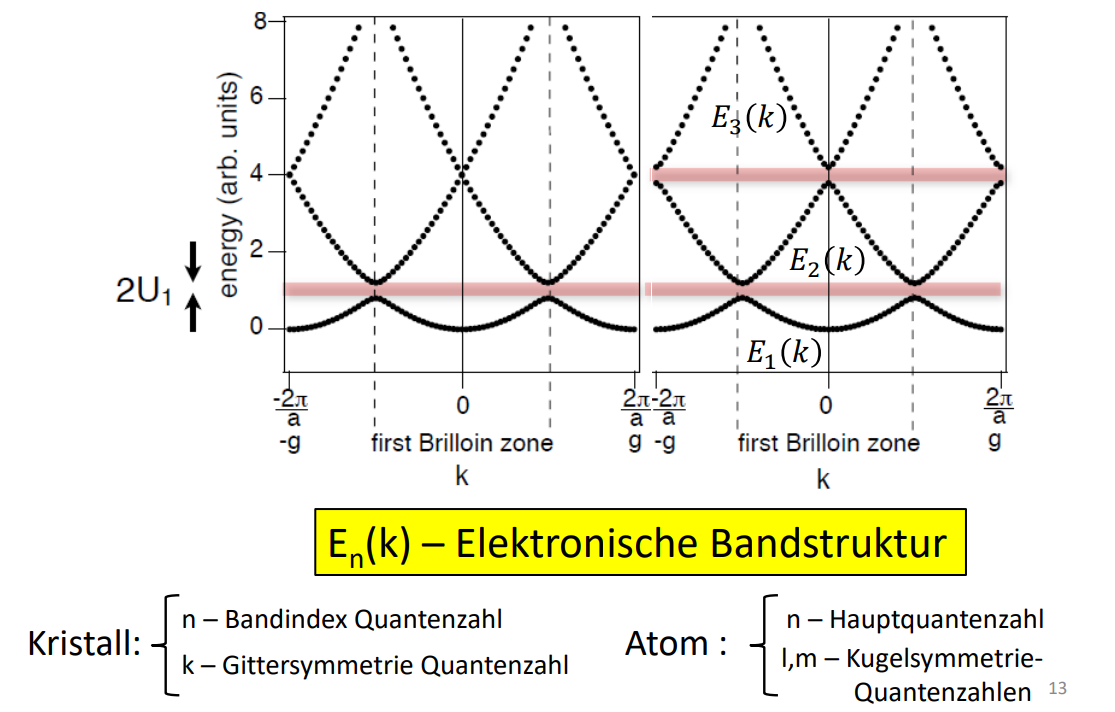
\includegraphics[width=6cm]{resources/05-05-2015/frage8_blochtheorem.PNG}
    \caption{Darstellung der Elektronischen Bandstruktur.}
\end{figure}

\question{Beschreiben Sie den Paulschen Paramagnetismus.}
\label{q:9}

\question{Potentiat-Bindung im homöopolaren Molekül?}
\label{q:10}

Siehe \aqref{q:11}.


\newpage
